\documentclass[a4paper,11pt,oneside]{book}

% --- CODIFICA E LINGUA ---
\usepackage[utf8]{inputenc}
\usepackage[T1]{fontenc}
\usepackage[italian]{babel}

% --- MARGINI E SPAZIATURA ---
\usepackage[top=2.5cm, bottom=2.5cm, left=2.5cm, right=2.5cm]{geometry}
\usepackage{parskip} % Spazio tra i paragrafi senza rientro
\usepackage{float}
\usepackage{bm}
\usepackage{tcolorbox}

\usepackage{graphicx}
% --- MATEMATICA E AMBIENTI TEOREMA ---
\usepackage{amsmath, amssymb, amsthm}
\theoremstyle{dispense}
\newtheorem{definizione}{Definizione}[chapter]
\newtheorem{teorema}{Teorema}[chapter]
\newtheorem{proposizione}{Proposizione}[chapter]
\newtheorem{lemma}{Lemma}[chapter]
\newtheorem{corollario}{Corollario}[chapter]
\newtheorem{osservazione}{Osservazione}[chapter]
\newtheorem{problema}{Problema}[chapter]
%--aggiunte table of contents--
\setcounter{tocdepth}{3}
\setcounter{secnumdepth}{3}
% Ambiente non numerato per gli Esempi
\newtheorem*{esempio}{Esempio}

% --- INTESTAZIONI E PIÈ DI PAGINA ---
\usepackage{fancyhdr}
\pagestyle{fancy}
\fancyhf{}
\renewcommand{\chaptermark}[1]{\markboth{Capitolo \thechapter.\ #1}{}}
\renewcommand{\sectionmark}[1]{\markright{\thesection.\ #1}}

\fancyhead[L]{\small\slshape\rightmark}
\fancyfoot[L]{\small\slshape\leftmark}
\fancyfoot[R]{\small\thepage}
\renewcommand{\headrulewidth}{0.4pt}
\renewcommand{\footrulewidth}{0.4pt}

% --- ALGORITMI ---
\usepackage{algorithm}
\usepackage{algpseudocode}
\floatname{algorithm}{Algoritmo}

% --- LINK CLICCABILI NELL'INDICE ---
\usepackage[hidelinks]{hyperref}

\begin{document}

% --- FRONTESPIZIO ---
\begin{titlepage}
    \centering
    \vspace*{2cm}

    {\large Dipartimento di Informatica}\\[3cm]
    {\Huge \bfseries Fisica}\\[0.5cm]
    {\Large Appunti integrati con il libro 'lezioni di fisica e termodinamica'}\\[4cm]
    \textbf{Autore}\\
    Giulia A. Gigante\\[1cm]
    \vfill
    {\large \today}
\end{titlepage}

\frontmatter
\tableofcontents

% --- CORPO DEL TESTO (Numerazione araba) ---
\mainmatter

\chapter{Galileo e il metodo scientifico}
\section{introduzione al metodo scientifico}
Con il suo 'cannochiale' Galileo notò che i mari della Luna, ovvero le chiazze scure che appaiono ad occhio nudo cambiavano al variare delle fasi lunari ne concluse quindi che la superficie lunare non era perfetta e sferica, ma conteneva montagne e crateri.\\
Ragionamento similare avvenne per quelli che oggi sono i satelliti di Giove che fino ad allora si pensava fossero stelle. Difatto nel gennaio del 1610 Galileo concluse che i pallini luminosi che ruotavano attorno a Giove come la Luna con la Terra erano bensì 4 satelliti. \\
Tale scoperta fu di fondamentale importanza per la teoria copernicana, fino a quel momento si dava fiducia infatti alla cosmologia aristotelica-tolemaica che vedeva al centro la Terra fissa e intorno in movimento i vari corpi celesti.
Copernico sosteneva invece che la Terra si muoveva attorno al Sole e la Luna attorno al sole. \\
Sempre per la cosmologia aristotelica, tutti i corpi celesti erano perfetti e sferici ma osservando Saturno al telescopio  Galileo osservò i rigonfiamenti al lato del pianeta (lo strumento dell'epoca non permetteva di distinguere gli anelli) egli lo interpretò nel seguente modo  \textit{ "....Saturno non è un astro singolo, ma è composto di tre corpi, e quello centrale è tre volte più  grande degli altri due..."}. \\
Solo nel 1659 Christiaan Huygens arrivò all' intuizione dell'anello intorno al pianeta.\\
Galileo osservò inoltre che Venere aveva un comportamento simile con il Sole  a quello della Luna con la Terra; osservò inoltre le macchie solari sul Sole.\\

\textbf{Tutte le osservazioni di Galileo confutavano la teoria tolemaica che prevedeva la terra al centro del sistema e la perfezione degli astri }
\newline

\begin{figure}[h!]
\centering
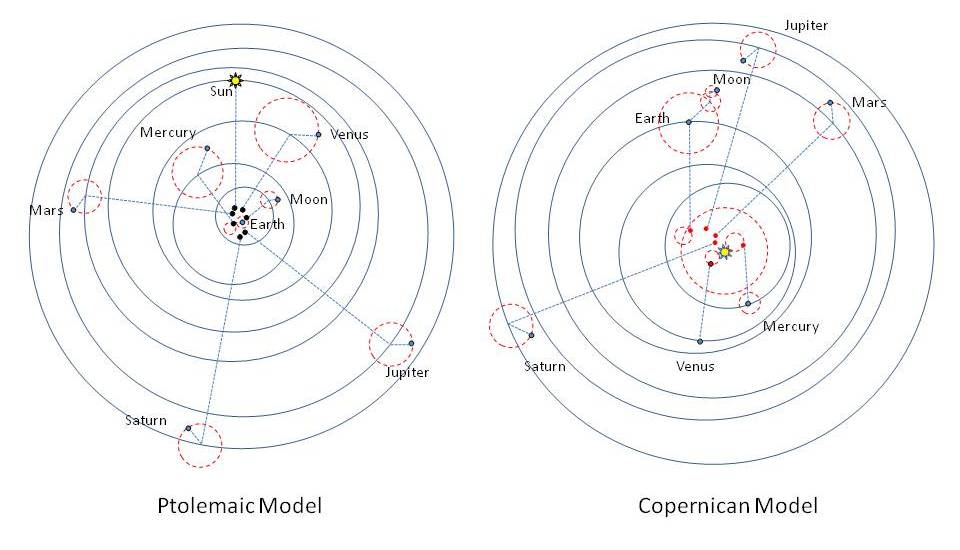
\includegraphics[width=0.5\textwidth]{immagini/tolomaico-copernicano}
\label{figura_1_sistematolocoper}
\end{figure}


\section{Strumenti, misurazioni oggettive e grandezze fisiche}
All'epoca non esistevano gli orologi come li conosciamo oggi , Galileo dovette cercare un modo per poter calcolare il tempo trascorso per i suoi esperimenti egli si accorse che l'oscillazione di un pendolo è indipendente dalla sua ampiezza (cosa vera solo per oscillazioni di piccola ampiezza). Galileo ebbe l'intuizione che si può costruire un orologio sfruttando il pendolo tuttavia non ci riuscii quindi per i suoi esperimenti egli utilizzo  gli orologi ad acqua.\\

\begin{figure}[H]
\centering
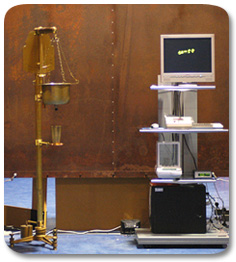
\includegraphics[width=0.3\textwidth]{immagini/orologioacqua_galileo}
\label{figura_2_orologio}
\end{figure}

Il funzionamento di un orologio ad acqua è particolarmente semplice si fa scorrere, come si vede in figura un flusso d'acqua ,  il tempo trascorso sarà quindi proporzionale alla quantità di acqua uscita.\\
\begin{definizione}[esperimento]
operazione o sequenza di operazioni con cui si intende riprodurre, simulare e determinare concettualmente un fenomeno, in modo che le sue condizioni siano note e riproducibili.\\
\end{definizione}

 \begin{definizione}[grandezze fisiche]
entità aventi una precisa definizione, utilizzabili per descrivere un fenomeno fisico, soggette a possibilità  di misura con relativa unità, per le quali valgono i criteri di uguaglianza e sommabilità. Le leggi fisiche esplicitano le relazioni
tra le grandezze fisiche necessarie per spiegare quantitativamente i risultati sperimentali di un fenomeno fisico.\\
\end{definizione}

Oltre ciò Galileo studiò anche il moto dei gravi  più precisamente la caduta libera di questi che, secondo la fisica aristotelica dell'epoca il loro moti erano determinati dal loro peso e dalla resistenza dell'aria .
Galileo come altri studiosi dell'epoca notare che due oggetti dello stesso materiale ma diverso peso lasciati cadere dalla stessa altezza arrivano a terra alla stessa velocità. Galileo riconosce \textit{l'effetto spurio dell'aria} . Negli anni successivi egli fece altri esperimenti e \textit{ne concluse} che tutti i corpi nel vuoto cadono ad accellerazione uniforme e  che la che la distanza che essi percorrono durante la caduta è proporzionale al quadrato del tempo impiegato per percorrerla.\\
\newline
Per lo studio della caduta dei gravi Galileo utilizzo il piano inclinato ,che gli permise di poter osservare meglio l'esperimento. Galileo riconosce che i due fenomeni seppur differenti sotto alcuni aspetti sono \textbf{equivalenti}.\\

Galileo quindi ipotizza una legge $ L \propto t^2$ che sta per la legge definita sopra, nonosrtante ciò sappiamo ad oggi che non è quella definitiva poichè la legge del \textbf {moto uniformemente accellerato} verrà trovato successivamente da Newton.\\

A questo punto Galileo notò che più era liscio il percorso su cui si faceva scendere il corpo sul piano inclinato più questo tendeva a fermarsi più tardi.  Questo lo portò all'intuizione sulla \textbf{ legge d'Inerzia} ovvero:  \textbf{lo stato di moto naturale di un corpo è quello del moto rettilineo uniforme a (velocità costante) indefinitamente}. 
\\
\\
Galileo ebbe un ultima intuizione, esaminando il moto dei proiettili egli si accorse che essi sono soggetti da due forze complessive quella lungo l'asse delle ascisse (la spinta dei proiettili e l'attrito dell'aria ) e quella lungo l'asse delle ordinate (la gravità), questo implica che le leggi del moto devono essere definite come vettori.

\section{Principio di relatività}
Seppur associamo comunemente la relatività a Einstein non è sbagliato associarla anche a Galileo anzi. Galileo infatti nota che si può descrivere un fenomeno solo se prima abbiamo definito il sistema di riferimento, le misure conseguite a tale fenomeno sono quindi relative al sistema di riferimento scelto
\\
esempio:
se lancio una pallina dentro a un treno in movimento per me la pallina ha velocità pari alla velocià datagli dal lancio \textit{w} ma per gianpirlo che vede il treno passare a velocità \textit{v} la pallina avrà velocità pari a \textit{v+w}, le misure fatte sono quindi relative al sistema di riferimento scelto.\\

\begin{definizione}[sistema di riferimento inerziale]
un sistema di riferimento si dice inerziale se in tale sistema di coordinate risulta valido il principio d'inerzia.\\
\end{definizione}

la relatività stabilisce che le leggi fisiche devono avere la stessa forma in sistemi di riferimento inerziali in moto relativo di traslazione tra loro. Questo è valido per la meccanica e per velocità piccole. 

\newpage
\chapter{Meccanica}
La meccanica studia il moto dei corpi e le cause che lo determinano, si usa comunemente suddividerla in cinematica dinamica e statica.
\begin{itemize}
\item \textbf{cinematica} $\to$ descrive il moto e le sue caratteristiche indipendentemente dalla cause.
\item \textbf{dinamica} $\to$ studia le cause che determinano un moto.
\item \textbf{statica} $\to$ studia il caso particolare dei corpi in quiete o in equilibrio 
\end{itemize}
\section{Cinematica}
Per poter trattare la cinematica esamineremo come caso di studio il \textbf{punto materiale} ovvero un oggetto di dimensioni e materiale trascurabile, in seguito vedremo anche i sistemi dei punti materiali; questi sono dei \textbf{modelli} ovvero delle schematizzazioni della realtà che ci permettono di descrivere più facilmente i fenomeni osservabili.\\
\subsection{sistema di riferimento e moti}
 Come detto prima è molto importante definire il sistema di riferimento poichè a seconda di questo un corpo si può trovare in stato di quiete o di moto. Per lo studio del moto di un punto materiale a ogni posizione assunta dal punto va associata un  \textit{ascissa temporale } fissando così l'istante dal quale iniziamo a misurare e così si può determinare gli istanti successivi e quelli che li precedono. \\
Il moto di un punto materiale nello spazio  è determinato quando è possibile conoscere la posizione ad ogni istante sapendo la dipendenza delle sue coordinate rispetto al tempo.
\noindent

\begin{minipage}{0.48\textwidth}
    \begin{equation*}
        \begin{cases}
	x=x(t)\\
	y=y(t)\\
	z=z(t)\\
	\end{cases}
    \end{equation*}
\end{minipage}
\begin{minipage}{0.48\textwidth}
    \centering
    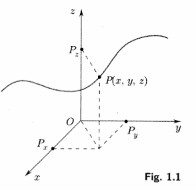
\includegraphics[width=0.3\textwidth]{immagini/spazio_cartesiano} 
    \label{figura_3_spazio_cartesiano}
\end{minipage}
\\
Ovviamente è possibile definire anche il vettore posizione che è dato da: \\ \bm{$\overrightarrow{r(t)}= x(t)\hat{i} + y(t)\hat{j} + z(t)\hat{k}$}.\\

Il punto materiale durante il suo moto descrive una linea nello spazio che prende il nome di \textbf{traiettoria}. Se la linea definita dal moto è una retta allora il moto si dice \textit{rettilineo}, un moto si dice \textit{piano }se la retta giace su un piano. Data la traiettoria è possibile definire un sistema di coordinate avente come origine \textbf{O} la posizione assunta dal punto \textbf{P} all'instante iniziale/zero, è chiaro che ora la conoscenza del moto è equivalente a conoscere  \textbf{s=s(t)} con  \textbf{s} rappresentante l'ascissa curvilinea.
\\

\subsubsection{moto rettilineo uniforme}
Supponiamo di voler osservare il moto rettilineo di un punto, è facilmente intuibile che lo spostamento da una ascissa $x_0$ a  ascissa x sia dato dalla seguente  uguaglianza \bm{$x=x_0+vt$} in cui \textbf{v} e \textbf{t} sono rispettivamente velocità scalare e tempo.\\
Nonostante ciò possiamo definire la velocità scalare in modo accurato nel seguente modo:\\

\begin{tcolorbox}
\begin{definizione}[velocità scalare]
la velocità scalare istantanea relativa allo stato di moto in un istante t  si definisce come il limite del rapporto s:

per $\Delta t = t_2 - t_1 \to 0$. Si ha
\[
  v_s = \lim_{\Delta t \to 0} \frac{x(t + \Delta t) - x(t)}{\Delta t}.
\]

\end{definizione}
\end{tcolorbox}

Si nota come la velocità scalare non sia nient'altro che la derivata rispetto al tempo della \textbf{x=x(t)} che esprime lo spazio percorso del punto materiale come funzione del tempo.\\
Nel moto uniforme la velocità scalare media coincide con la velocità scalare istantanea.\\

possiamo quindi arrivare alla seguente uguaglianza:\\
\begin{tcolorbox}
\[ \lim_{\Delta t \to 0} \frac{\Delta \mathbf{r}}{\Delta t} = \frac{d\mathbf{r}}{dt} = \mathbf{i} \frac{dx(t)}{dt} = \mathbf{i} \dot{x} = \mathbf{i} v
\]
\end{tcolorbox}
la quale rappresenta il vettore velocità del punto \textbf(P) all'istante(t) e  \bm{$\delta r$} rappresenta ($x_2 - x_1$) e \bm{$\delta t$} rappresenta ($t_2-t_1$). Perciò la velocità scalare è la componentedi v lungo l'asse delle ascisse .
Inoltre \textit{la velocità vettoriale risulta essere un vettore dimtto secondo la tangente alla traiettoria nella posizione occupata dal punto materiale all'istante in considerazione, avente il verso del moto, e come intensità il valore assoluto v della velocità scalare}.\\

Le dimensioni della velocità sono:\\
\[
  \bm{[v]=[LT^-1]}
\]

Adesso definiamo il sistema di equazioni che ci permette di definire  il moto rettilineo uniforme
\begin{equation}
\begin{cases}
V(0)=V_0,   \quad  a=0\\
x(t)=x_0 + V_0(t-t_0)\\

\end{cases}
\end{equation}

\subsubsection{moto uniformemente accellerato}
Supponiamo ora di voler aggiungere a questo moto un accelerazione costante, questo implica che più tempo passa più la velocità. definiamo l'accelerazione nel seguente modo:
\begin{tcolorbox}
\begin{definizione}[accellerazione]
Si considerino due istanti $t_1$ e $t_2$ ($\Delta t = t_2 - t_1$) e siano $P_1$ e $P_2$, $V_1$ e $V_2$ le posizioni corrispondenti sull'asse $x$ del punto materiale e le relative velocità vettoriali. Data la variazione della velocità $\Delta \mathbf{v} = \mathbf{v}_2 - \mathbf{v}_1$ nell'intervallo $\Delta t$, si definisce accelerazione vettoriale $\mathbf{a}$ il vettore:
\[
  \mathbf{a} = \lim_{\Delta t \to 0} \frac{\Delta \mathbf{v}}{\Delta t} = \frac{d\mathbf{v}}{dt}
\]
ricordando la definizione di velocità come derivata dello spazio rispetto al tempo otteniamo che:
\[
  \mathbf{a} = \frac{d\mathbf{v}}{dt} = \mathbf{i} \ddot{x}(t) = \mathbf{i} \frac{dv_s(t)}{dt} = \mathbf{i} a_t
\]
in cui $\ddot{x}$(t) rappresenta la derivata seconda rispetto al tempo dello spazio.
\end{definizione}
\end{tcolorbox}
Le dimensioni dell'accellerazione sono:\\
\[
  \bm{[a]=[LT^-2]}
\]
Quindi il vettore accellerazione è la derivata prima temporale del vettore velocità o anche la derivata seconda temporale del vettore spostamento.
\\
Possiamo ora definire le equazioni del moto uniformemente accellerato
\begin{equation}
\begin{cases}
V(t)=a_0(t-t_0)+V_0\\
x(t)=x_0 + V_0(t-t_0)+ \frac{1}{2}a_0(t-t_0)^2\\

\end{cases}
\end{equation}
Ovviamente possiamo definire la velocità in un nuovo modo a partire dall'accellerazione:
\begin{tcolorbox}
\begin{definizione}[velocità come integrale dell'accellerazione]
\[
  y = \int_{0}^{t} v \, dt = y_0 + v_0 t + \frac{1}{2} a_t t^2.
\]
\end{definizione}
\end{tcolorbox}
\newpage
nella figura qui sotto sono rappresentati tre grafici che rappresentano in ordine lo spostamento, la velocità e l'accelerazione.\\

\begin{figure}[H]
\centering
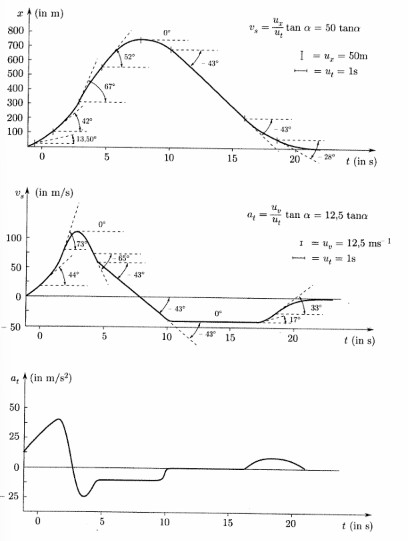
\includegraphics[width=0.5\textwidth]{immagini/grafico_vel_acc_spazio}
\label{figura_4_graficimotorettiuniacc}
\end{figure}
\begin{esempio}
Supponiamo di avere $t_1 = 3,4\text{ s}$ e $V(t_1) = 100\text{ km/h}$ (che sono equivalenti a $27,7\text{ m/s}$) e sappiamo che la velocità iniziale $V_0$ è pari a $0$. Vogliamo sapere quanto vale l'accelerazione \quad iniziale $a_0$.\\
\small\textit{(Dalla formula precedente possiamo scrivere la seguente uguaglianza:)}
\[
  a_0 = \frac{V(t_1) - V_0}{t_1 - t_0} = \frac{27,7\text{ m/s} - 0}{3,4\text{ s} - 0} = 8,17\text{ m/s}^2
\]
\end{esempio}
Definiamo ora un accellerazione molto conosciuta, l'\textbf{accellerazione gravitazionale} definita come vettore verso il basso rispetto a un sistema di coordinate in cui l'y va verso l'alto  essa ha misura definita nel seguente modo: \[  \vec{g} = -9{,}81 \, \text{m/s}^2 \, \hat{y}\]

Quindi per un oggetto in caduta perpendicolare all'asse delle x possiamo definire un sistema di equazioni rappresentante il moto nel seguente modo:
\begin{equation*}
\begin{cases}
y(t)=y_0+ V_0t -\frac{1}{2}gt^2\\
V_y=V_0-gt
\end{cases}
\end{equation*}

Questa equazione è molto utile se si vuole trovare il momento in cui  l'altezza è massima per cui la direzione della velocità cambia direzione e il punto/oggetto inizia a tornare verso il basso. Per trovarla occore eguagliare la seconda equazione a 0, infatti nel momento che la velocità cambia direzione implica che questa deve essere uguale alla velocità creata dall'accellerazione gravitazionale in quel momento.\\

\subsubsection{moto circolare uniforme}
\begin{definizione}[radiante]
unità di misura degli angoli piani nel SI, è definito a partire dall’angolo al centro di una circonferenza; è l’ampiezza di quell’angolo al centro che sottende su tale circonferenza un arco di lunghezza uguale al suo raggio. per calcolare quanto un angolo in gradi vale in radianti si può utilizzare la seguente proporzione:
\[
  g : 180^\circ = x : \pi
\] un radiante vale all'incirca 57,3 gradi.
\end{definizione}
il moto circolare uniforme è così definito poiche avviene su una traiettoria circolare come  mostrato in figura.\\
\begin{minipage}{0.48\textwidth}
Si definisce la velocità scalare come la derivata prima della lunghezza dell'arco percorso rispetto al tempo. La velocità sarà diretta lungo la tangente nel verso del moto , e cambia direzione ad ogni istante.
definiamo ora la velocità angolare $\omega$, esaminiamo d'apprima la seguente proporzionalità :
sia  L(t)=R$\varphi$ con R il raggio della circonferenza allora si ha anche  che $\dot{L}(t) = R \dot{\varphi}(t)$
\end{minipage}
\begin{minipage}{0.48\textwidth}
    \centering
    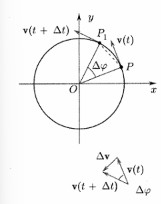
\includegraphics[width=0.4\textwidth]{immagini/motocircolareuni} 
    \label{figura_5_moto_circolare}
\end{minipage}
che ci permette di ottenere  la seguente uguaglianza $\dot{\varphi}(t) = \frac{d\varphi(t)}{dt} = \omega$
$\omega $ sarà proprio la velocità angolare scalare  e si misura in \textit{radianti} al secondo, risulta elementare capire che la velocità angolare ha intensità pari alla derivata temporale dell'angolo descritto dal punto. Il vettore della velocità angolare avrà direzione  lungo l'asse di rotazione e  il verso si determina con la regola della mano destra.\\
Il sistema di equazioni che lo descrive è il seguente:
\[
\begin{cases}
  x(t) = R \cos(\omega t) \\
  y(t) = R \sin(\omega t)
\end{cases}
\]
Il moto è periodico possiamo definire quindi le seguenti tre formule:\\
\begin{itemize}
\item$ \omega=\frac{v}{R} \quad (velocità angolare)$
\item $T=\frac{2\pi R}{v} \quad (periodo)$
\item  $\omega= \frac{2\pi}{T}$
\end{itemize}

L'accellerazione nel moto circolare uniforme è definita come il limite per $\delta t $ che va 0 per$ \delta$ v fratto $\delta t  \longrightarrow  a=  \lim_{\Delta t \to 0}\frac{\delta v}{\delta t} $\\
si dice quindi che l'accellerazione è normale a v(t) ed è diretta in ogni punto verso  il centro della traiettoria stessa, l'accellerazione può essere scomposta in due componenti una tangente alla curva e l'altra che punta verso il centro , quella verso il centro è chiamata centripeta/normale.
\subsubsection{moto diverso}
Esaminiamo un moto che ha come traiettoria una linea qualsiasi allora per scomporre l'accellerazione in un punto è utile usare un cerchio osculatore
\begin{definizione}[cerchio osculatore]
si definisce come cerchio osculatoe  un cerchio tangente a un punto della traiettoria e che ha il centro sulla normale, difatto la normale sarà il raggio del cerchio.

\end{definizione}
%%aggiungi la foto del tablet
\subsection[Leggi di Newton]
Le leggi di Newton o anche detti principi della dinamica sono  tre leggi fondamentali della fisica che descrivono il legame tra il moto di un corpo e le forze che agiscono su esso
\begin{itemize}
\item \textbf{legge d'Inerzia} $\longrightarrow$ Un corpo rimane nello stato di quiete o di moto rettilineo uniforme a meno che non intervenga una forza esterna attua a modificarne lo stato 
\item \textbf{principio di conservazione} $\longrightarrow$ l'accellerazione di un corpo è direttamente proporzionale alla forza netta applicata e inversamente proporzionale alla sua massa  \textbf{$\vec{F}=m\frac{d\vec{v}}{dt}$}
\item \textbf{Principio di azione e reazione} $\longrightarrow$ se un corpo A esercita una forza su un corpo B allora il corpo B esercita una forza uguale e contraria , [F]=[ml$t^-2$]=N con N letto come Newton
\end{itemize}

\subsection{Forze d'attrito}


\end{document}
